\IfFileExists{assets/latex/IEEEtran.cls}
  {\documentclass[conference]{assets/latex/IEEEtran}}
  {\documentclass[conference]{IEEEtran}}  % overleaf has it built in
\IEEEoverridecommandlockouts

\usepackage{amsmath,amssymb,amsfonts}
\usepackage{graphicx}
\usepackage{textcomp}
\usepackage{xcolor}

\graphicspath{{assets/latex/}}

\begin{document}

\title{CS6524 Computer Vision Lab. 3\\ Structure from Motion}

\author{\IEEEauthorblockN{Dylan Teehan}}

\maketitle

\begin{abstract}
I filmed a football boot on a stool twice with my iPhone, once walking around it and once with the phone still while I spun the stool. From each video I worked out where the camera was in every frame and built a 3D point cloud. The first video worked well and the stool and boot come out clearly. The second only partly worked. Changing the focal length bent the shape of the cloud, even though the error numbers barely changed.
\end{abstract}

\section{Methodology}

\subsection{Recording}
Video a walks the camera 360\textdegree{} around the boot, and video b keeps the phone still while the stool turns. Both were shot on camera 2 from lab 2 (iPhone 13 Pro) and shrunk to $360\times640$ at 30\,fps with the same script as the calibration video, so I could reuse its $K$ and $D$. I used every 10th frame, as back-to-back frames barely moved.

\subsection{Keypoints and tracks}
I tried SIFT and ORB. SIFT found a camera for every frame of video a, and ORB lost about a quarter of them, so I used SIFT. I matched each frame to the next one and linked the matches into tracks, so the same point keeps one ID across frames. Most tracks only last 2 or 3 frames, so I kept every track seen at least twice instead of only the long ones, which would have left almost nothing.

\subsection{Camera poses}
The first two frames give the essential matrix, which gives the rotation $R$ and direction of movement $t$, like in lab 2. After that I did not keep using essential matrices, as each pair would come out at a different scale. Instead each new frame is placed with PnP against the 3D points I already had. Every point is worked out from all the frames that see it, and points that land behind a camera or more than 2\,px off are thrown out. Every 5 frames I redo the points and adjust the last 10 cameras so small errors do not build up around the circle.

\subsection{Video b}
A boot spinning in front of a still camera looks the same to the maths as a camera walking around a still boot. The background does not move though, so I ignore points that move less than 3\,px between frames. I also skip frames where my spin paused, since no movement means no pose.

\subsection{Dense cloud and sensitivity}
Once every camera is placed, I rectify each pair of frames, use StereoSGBM to get depth like in lab 2, and put every pixel into 3D. Points that land in the same small cube are averaged, and cubes with fewer than 3 points are dropped as noise. I then reran everything with the focal length times 0.8, 1 and 1.2, with and without undistortion, which gives the 12 point clouds.

\begin{table}[t]
\caption{Results per run (08/10/12 is the focal length factor, u is undistorted, d is not)}
\begin{center}
\begin{tabular}{|l|c|c|c|}
\hline
\textbf{Run} & \textbf{Frames placed} & \textbf{Error (px)} & \textbf{Points} \\
\hline
a\_08u & 55/84 & 0.40 & 165k \\
a\_08d & 84/84 & 0.40 & 206k \\
a\_10u & 84/84 & 0.32 & 127k \\
a\_10d & 84/84 & 0.31 & 132k \\
a\_12u & 84/84 & 0.33 & 147k \\
a\_12d & 84/84 & 0.39 & 188k \\
\hline
b\_08u & 6/17 & 0.42 & 108 \\
b\_08d & 13/17 & 0.39 & 58k \\
b\_10u & 13/17 & 0.29 & 70k \\
b\_10d & 6/17 & 0.34 & 33k \\
b\_12u & 12/17 & 0.38 & 28k \\
b\_12d & 12/17 & 0.37 & 63k \\
\hline
\end{tabular}
\label{tab:runs}
\end{center}
\end{table}

\begin{figure}[t]
\centerline{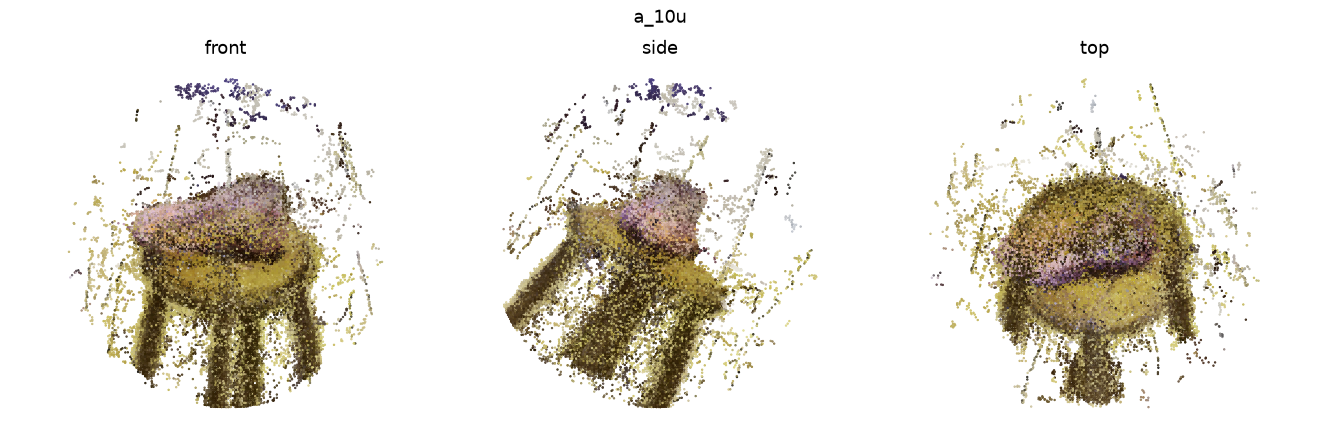
\includegraphics[width=\columnwidth]{a_10u.png}}
\caption{Video a from the front, side and top. You can see the four legs of the stool and the pink boot on top.}
\label{fig:a}
\end{figure}

\begin{figure}[t]
\centerline{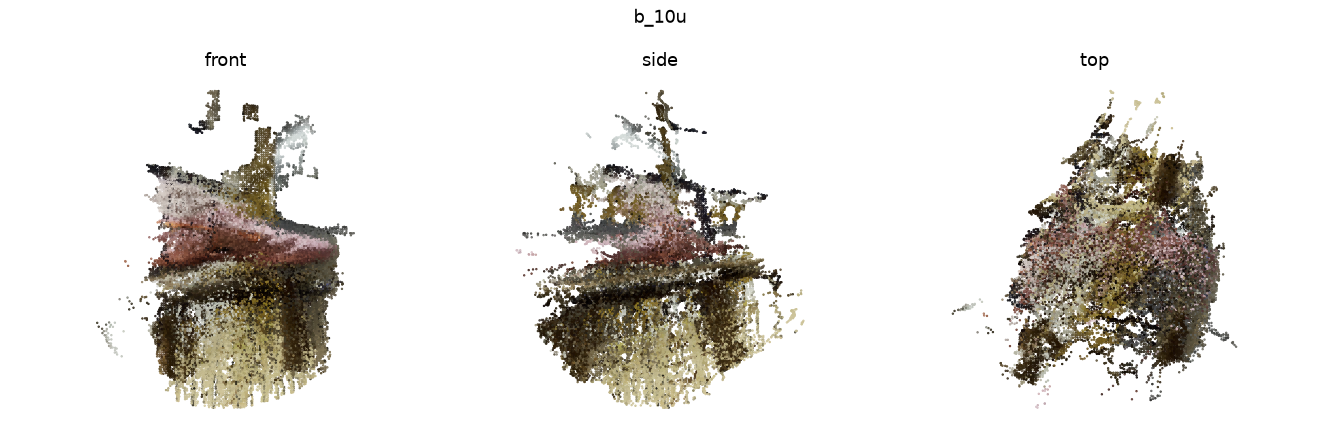
\includegraphics[width=\columnwidth]{b_10u.png}}
\caption{Video b from the front, side and top. The boot is there but the cloud only covers part of the turn.}
\label{fig:b}
\end{figure}

\begin{figure}[t]
\centerline{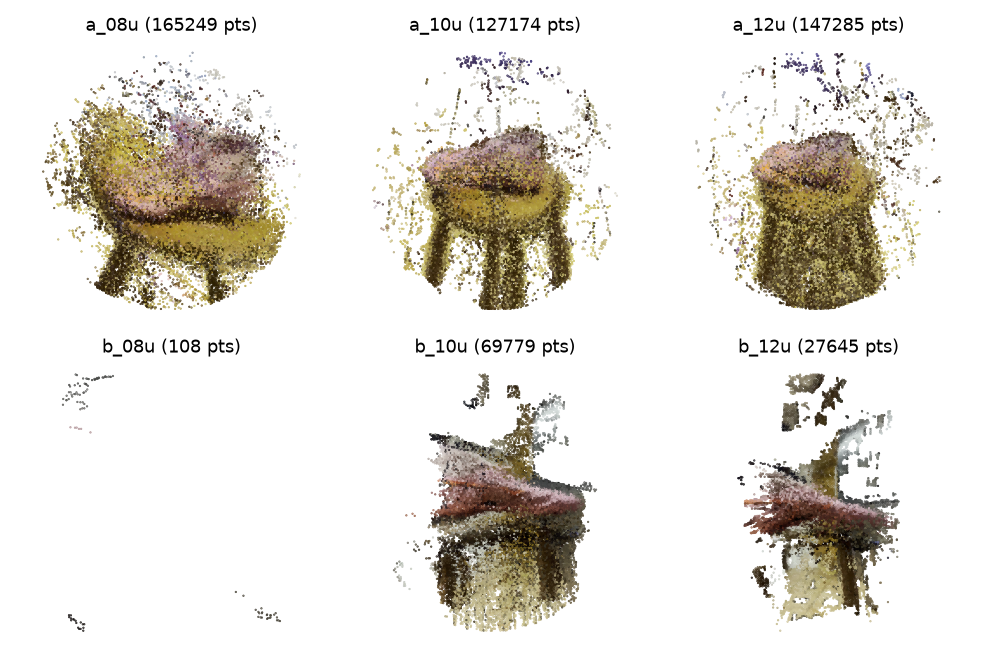
\includegraphics[width=0.8\columnwidth]{sensitivity.png}}
\caption{Front view at focal length times 0.8, 1 and 1.2. At 0.8 the stool bends, and at 1.2 the legs merge.}
\label{fig:sens}
\end{figure}

\section{Results}
Fig.~\ref{fig:a} shows video a. Every frame got a camera and the stool and boot look right from every side. Fig.~\ref{fig:b} shows video b, where the boot is there but only 13 of 17 frames got a camera. Table~\ref{tab:runs} shows all 12 runs and Fig.~\ref{fig:sens} shows what the focal length does.

\section{Discussion}

\subsection{What worked}
Video a worked best. The stool comes out with four separate legs, which means the cameras were placed in the right spots. The stool shows up as well as the boot because anything that stays still while the camera moves gets rebuilt. Like lab 2, the cloud has no real scale.

\subsection{The focal length}
This surprised me most. With the wrong focal length the error barely changed, but the shape did. The focal length decides how wide each pixel's view is. Too small and the camera seems to turn more than it did between frames, too big and it seems to turn less. The cameras and points then fit those wrong angles, so the error stays low but the stool bends. A low error only means the result agrees with the $K$ I gave it, not that it is right.

\subsection{Other problems}
Undistortion barely changed anything, I think because the boot is near the middle of the frame where the lens bends things least.

My first video b failed after 2 frames, as the smooth pink boot had very few points to match. Filming closer helped but it still breaks partway round. I think the lighting is the main reason. In video a only the camera moves, so the boot looks the same in every frame. In video b the boot turns under the light, so its shading keeps changing and matches get worse.

At first the whole thing stopped at frame 3. The mask from \texttt{recoverPose} was throwing away almost every point, and using the RANSAC mask instead fixed it.

\subsection{Next steps}
\begin{enumerate}
\item Match each frame to the one two ahead too, so one bad frame does not stop everything.
\item Match the last frame to the first, since both videos go all the way round.
\item Refine all cameras and points together at the end.
\item Re-film video b on a patterned surface with even lighting.
\end{enumerate}

\end{document}
